\chapter{Local Feature Extraction}
In this chapter we will provide you a couple of additional feature sets that are commonly used in computer vision applications.
More specifically, we are talking about the local features extraction modules. 
First, we define it \textit{local} because the features points are extracted not at an object level, but from little patches. 
So we are not considering the whole object, but only a small part of it that can help to characterize the object itself such as intensity and direction of edges.
\\
In particular, we will focus on two different algorithms: HOG and SIFT.
\section{HOG}
The first algorithm we are going to introduce is the Histogram of Oriented Gradients.
We already know that gradient is what characterizes the edges of an image, where the edge means that we are dealing with the transition from a gray level to another one.
In the Histogram of Oriented Gradients we can easily recognize the object in the image by looking at the vectors. The stronger the gradient, the brighter the arrow will be.
While where the edges are weaker the arrow will be less intense.

\begin{figure}[H]
    \centering
    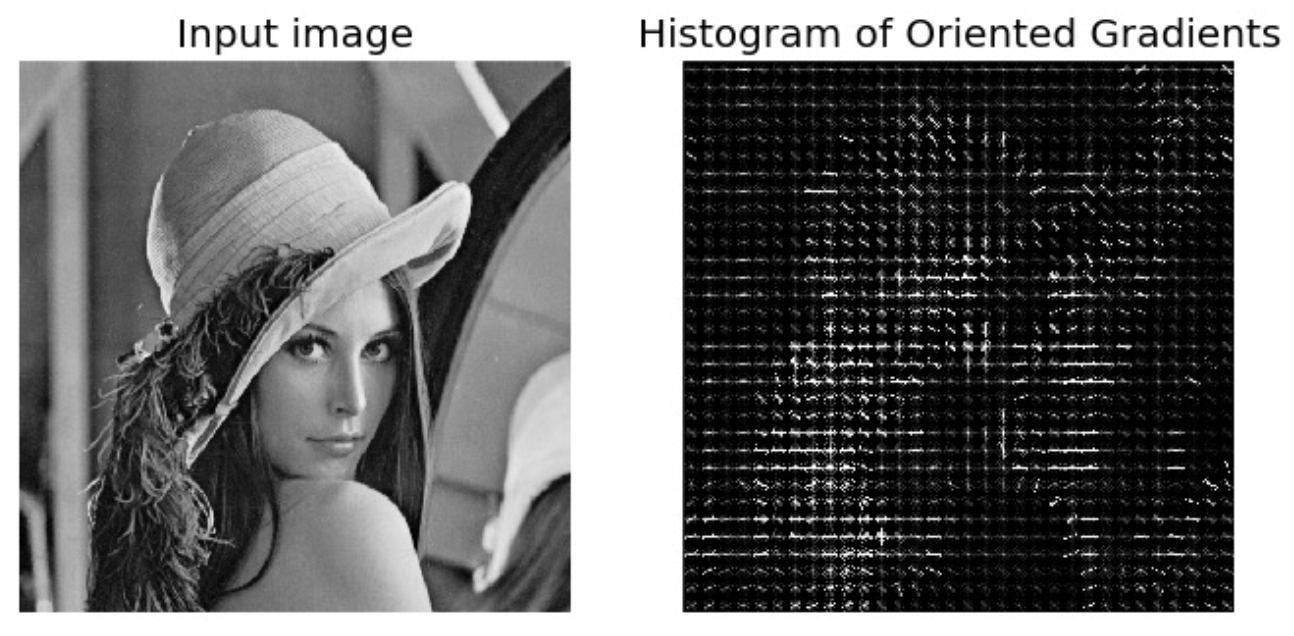
\includegraphics[width=0.5\textwidth]{Figures/HOG.png}
    \caption{Vector representation of the gradients in an image.}
    \label{fig:HOG}
\end{figure}

So basically, what we are doing inside the picture is to divide it into small patches and look at the gradient of each pixel in the patch.
Then we characterize those gradients using a direction information and a magnitude or intensity.
At the end of the process we can construct a descriptor which can be used by next algorithms to recognize the presence of object in the image.
\\But how do we get the descriptor?
First of all, we need to divide the image into a number of rectangular or radial cells of arbitrary size.
\\\textit{NB: It's good practice to have only one main edge component inside a cell, so small cells are preferable.} 
\\Then, for each pixel in the cell we compute the orientation of edge(\textit{Take a pixel, take his neighbor and see if there is an edge or not}), which gets subsequently quantized and put in one of the histogram's bins.
This means that each pixel within the cell can cast a vote, weighted by the gradient magnitude, for an orientation histogram based on the values found in the gradient computation.
In other words, each cell is represented through a 1D array (that corresponds to the bins of the histogram) that describes the gradient direction of the cell.
In addition, intensity is locally normalized in the RGB or LAB color space using L1 or L2-norm, to account for illumination changes and shadowing especially when using larger areas (blocks), consisting of more cells.
\\Just to wrap up, let's take a look to the pipeline:
\begin{figure}[h]
    \centering
    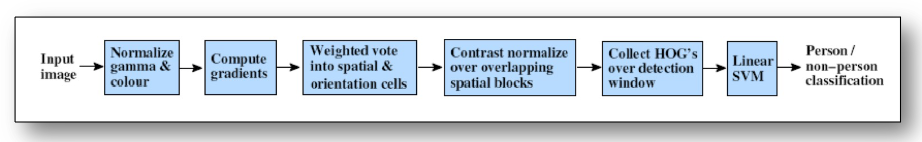
\includegraphics[scale=0.45]{Figures/HOG_Pipeline.png}
\end{figure}
\\It basically consists of taking the input image, computing the gradients and then the voting for each pixel, applying some additional normalization and finally getting the descriptor.

But what does it mean having a descriptor? It means that, for an object, we have a full description of its shape, obtained by concatenating all the cells, where each cell represents the gradient information within a small patch of the image.

Once we have our descriptor, we can pass it to a classifier, such as an SVM as you can see from the pipeline, to perform tasks like human detection. 
\\
Since this is not a machine learning course, we will just take a quick look at the \textbf{Dalal and Triggs algorithm}, a popular method for human detection available in OpenCV:

\begin{itemize}
    \item Arrange the data in a $64\times128$ window;
    \item Divide the window into $8\times8$ pixel cells;
    \item Blocks are formed by grouping $2\times2$ cells;
    \item Each cell has a histogram of 9 directions;
    \item The final descriptor is formed by concatenating the feature elements from these cells in each block, so a 36D vector.
    \item Blocks overlap to allow a smoother transition across the different blocks. In a $64\times128$ window we can fit $7\times15$ blocks.
\end{itemize}

\begin{wrapfigure}{r}{0.45\textwidth}
    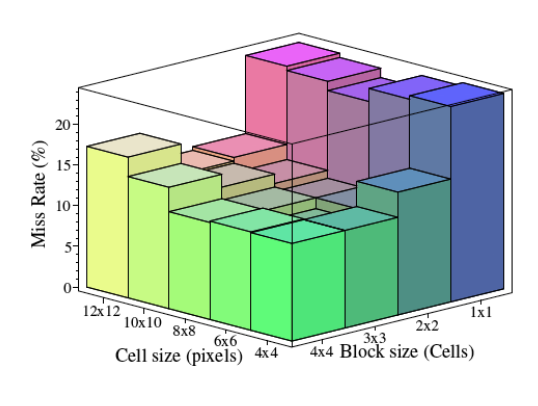
\includegraphics[scale=0.3]{Figures/Performance.png}
    \caption{Performance of the HOG algorithm with different configurations.}
    \label{fig:Performance}
\end{wrapfigure}
This configuration was chosen based on performance tests that measured the miss rate. As depicted in Figure \ref{fig:Performance}, this specific setup achieved the best results. Therefore, when implementing similar algorithms, we suggest to use overlapping blocks with a relatively high number of orientation bins and a moderate size of the elements you use.
\subsection{The problem of scale}
The problem of scale is a common issue even in current classifiers. The fact is that in video the pedestrian can be detected at different sizes.
This can be due to the spacial resolution of the camera, the distance from the object and even the object itself.
So, how can we solve this problem? A possible solution is to use a multiscale approach. This means that we need to resize the window at different scales and then apply the algorithm on all different sizes.
\subsection{Feature compression}
The last thing we want to mention is the feature compression. The descriptor can be very large, so we need to compress it in order to reduce the computational cost for delivering.
\\\textit{NB: To compute the compression in a lossless way, we can extract the histograms.}
\begin{figure}[h]
    \centering
    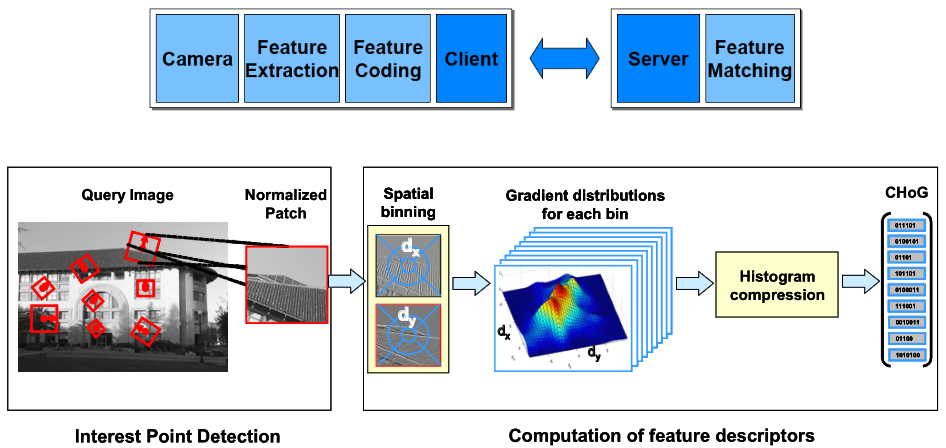
\includegraphics[scale=0.5]{Figures/FeatureCompression.png}
\end{figure}
\\Let's explain a little bit.
\\We compute the histograms and quantize them, so at this point we have just a few numbers that represent the descriptor. 
We (client) send them to the server that has a huge database filled up with the information of blocks, objects, songs, etc.
The server takes the features and compares them with the database, then it returns the result.
So, in terms of computation, what we are doing is called spatial binning.

% TODO: integrate some more about the compression of the features, encoding etc

\section{SIFT}
The Scale Invariant Feature Transform is an algorithm that extract the salient points of an image, points that exhibit certain proprieties. The Good Features to Track algorithm just extracts corners, and corners by themselves are not enough to \textit{describe} an object, in SIFT case we want to use these features in order to come up with objects' representations made up from a concatenation of features.
The main idea is to find the key-points that are \textbf{invariant to scale}, rotation, illumination and viewpoint changes.
The algorithm is composed by four main steps:
\begin{itemize}
    \item construct a subspace representation of the image by progressively apply a Gaussian(low pass) smoothing filter;
    \item at every iteration, each image becomes a blurred version of the previous one. This because, since we are looking for \textit{strong} points, a strong point should survive blurring operations;
    \item find key-points;
    \item compute the descriptor.
\end{itemize}
The filtering is obtained by applying a regular Gaussian filter to the image:
\[
    L(x,y,\sigma) = I(x,y) * \frac{1}{2\pi\sigma^2}e^{-\frac{x^2+y^2}{2\sigma^2}}
\]
where $I(x,y)$ is the image, $L(x,y,\sigma)$ is the scale space of the image after convolution and $\sigma$ is the standard deviation of the Gaussian filter (strength of the filter).
\\\textit{NB: A large sigma means a strong filter, which will tend to average more points.}

The next step is a procedure called the \textbf{creation of octaves}. An octave is a set of images of the same size where each image is a blurred version of the previous one. The next octave is obtained by downsampling the original image by a factor of $2$, we can crate octaves iteratively as long as the image can be downsampled.

\begin{figure}[H]
    \centering
    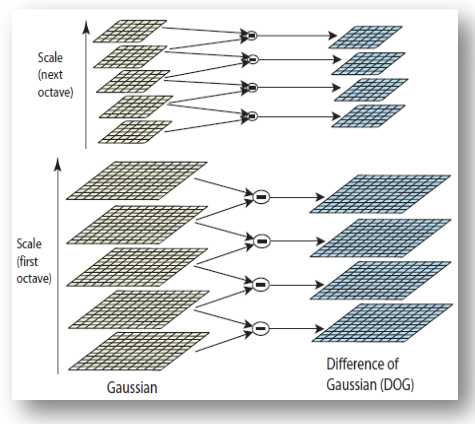
\includegraphics[scale=0.5]{Figures/dog.png}
    \caption{Difference of Gaussian}
    \label{fig:dog}
\end{figure}

Having the filtered version of the image, we can create the Difference of Gaussian (DoG) by subtracting, for each pair, the blurred image from the previous one as shown in Figure \ref{fig:dog}.
More generally, we are trying to \textit{highlight what survives} subtraction after subtraction, so we are looking for the maximum and minimum of the DoG.

\begin{figure}[H]
    \centering
    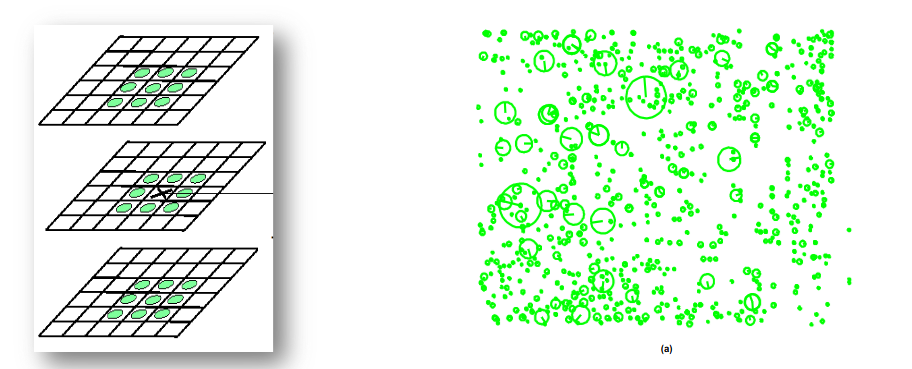
\includegraphics[scale=0.4]{Figures/dogs2.png}
    \caption{Selection of pixels among the DoGs.}
    \label{fig:dogs2}
\end{figure}

To grab the most salient points from the DoGs, each pixel from a given DOG is compared to its 26 neighbors ($8$ in the same scale, $9$ above and $9$ below).
A pixel is kept as a key-point only if it is greater (maximum) or smaller (minimum) than its neighbors.

DoG function exhibits strong response to edges, but edges are not always good key-points, the selection of the points might be noisy, so we can apply a second order Taylor expansion with the derivative set to $0$. 
\[
    D(X)=D + \frac{\partial D^T}{\partial X}X + \frac{1}{2}X^T\frac{\partial^2D}{\partial X^2}X
\]
Through this derivative we can obtain the maximum and minimum and construct a Hessian matrix $H$.
The Hessian matrix is the one that told us if the point that we have found are actually good or not.
Having it we can construct the trace and the determinant of the matrix to define a threshold.
\[
    H = \begin{bmatrix}
        D_{xx} & D_{xy} \\
        D_{yx} & D_{yy}
    \end{bmatrix}
\]
What we can check at this point is the ratio between the determinant and the trace of the matrix.
If the ratio is greater than a certain threshold, we can consider the point as a key-point.
So now consider $r = \frac{\alpha}{\beta}$, where $\alpha$ and $\beta$ are the largest and smallest eigenvalues in magnitude of the Hessian matrix.
If \[ \frac{Tr(H)^2}{Det(H)} < \frac{(r+1)^2}{r} \] is satisfied, then the point is a key-point.
\\
But not only, we can also check the magnitude and the orientation of the gradient.
This is because the eigenvalues of H are proportional to the curvature of the function D, so if the curvature is high in both dimensions, the gradient and orientation are computed.
This step achieves the invariance to rotation:
\[
    m(x,y) = \sqrt{(L(x+1,y)-L(x-1,y))^2 + (L(x,y+1)-L(x,y-1))^2}  
\]
\[
    \theta(x,y) = \arctan\left(\frac{L(x,y+1)-L(x,y-1)}{L(x+1,y)-L(x-1,y)}\right)
\]
The region within which $m$ and $\theta$ are computed is relative to the scale of the key-point, the higher the scale, the larger the computation region.
\\\textit{NB: This is very helpful for us to match the points across different images with different scale and resolution.}
\\
Then, from the orientations, a 36-bin histogram is computed. If a key-point exhibits multiple peaks in the histogram that are higher than $80\%$ of the highest peak, a new key-point is instantiated with same location and scale.
The 16x16 area (oriented according to the key-point orientation computed before) around the selected key-point is divided in $4\times4$ regions, and for each of them a histogram of the gradients (8bins) is computed.
This turns out in a descriptor of 128 elements ($4\times4\times8$).
\\
Once that the descriptor is constructed, we can use it to search and match the key-points in different images. This is done usually by Nearest Neighbor searching, where the Euclidean distance between the descriptors is computed, or by using optimization algorithms like RANSAC. 